\documentclass[12pt]{article}
\usepackage{amsmath}
\usepackage{amssymb}
\usepackage[letterpaper,top=0.85in,bottom=1in,left=0.75in,right=0.75in,centering]{geometry}
%\usepackage{fancyhdr}
\usepackage{enumerate}
%\usepackage{lastpage}
\usepackage{multicol}
\usepackage{graphicx}

\reversemarginpar

%\pagestyle{fancy}
%\cfoot{}
%\lhead{Math 1560}\chead{Test \# 1}\rhead{May 18th, 2017}
%\rfoot{Total: 10 points}
%\chead{{\bf Name:}}
\newcommand{\points}[1]{\marginpar{\hspace{24pt}[#1]}}
\newcommand{\skipline}{\vspace{12pt}}
%\renewcommand{\headrulewidth}{0in}
\headheight 30pt

\newcommand{\di}{\displaystyle}
\newcommand{\abs}[1]{\lvert #1\rvert}
\newcommand{\len}[1]{\lVert #1\rVert}
\renewcommand{\i}{\mathbf{i}}
\renewcommand{\j}{\mathbf{j}}
\renewcommand{\k}{\mathbf{k}}
\newcommand{\R}{\mathbb{R}}
\newcommand{\aaa}{\mathbf{a}}
\newcommand{\bbb}{\mathbf{b}}
\newcommand{\ccc}{\mathbf{c}}
\newcommand{\dotp}{\boldsymbol{\cdot}}
\newcommand{\bbm}{\begin{bmatrix}}
\newcommand{\ebm}{\end{bmatrix}}                   
                  
\begin{document}


\author{Instructor: Sean Fitzpatrick}
\thispagestyle{empty}
\vglue1cm
\begin{center}

{\bf MATH 1560 - Tutorial \#1 Solutions}\\

\end{center}



\textbf{Additional practice:}
\begin{enumerate}
\item Given $f(x)=\sqrt{x}$, $g(x)=x^2$, and $h(x)=e^{2x}$, compute:
\begin{enumerate}
\item $f(f(x)) = \sqrt{\sqrt{x}}=(x^{1/2})^{1/2} = x^{1/4} = \sqrt[4]{x}$.
\item $f(g(x)) = \sqrt{x^2} = \abs{x}$.

Note that it is only true that $\sqrt{x^2}=x$ when $x\geq 0$. The function $f(x)$ is the \textit{positive} square root function. If $x<0$ we have $\sqrt{x^2}=-x$. For example, if $x=-2$, then $x^2=4$, and $\sqrt{x^2} = \sqrt{4} = 2 = -(-2) = -x$.
\item $g(f(x)) = (\sqrt{x})^2 = x$.

Here we do get back $x$. Note, however, that the domain of this function includes only $x\geq 0$, since the square root of a negative number is not a real number.
\item $g(h(x)) = (e^{2x})^2 = e^{2(2x)}=e^{4x}$.
\item $h(f(x)) = e^{2\sqrt{x}}$.
\end{enumerate}


\item Determine if the function is even, odd, or neither:

\begin{enumerate}
\item $f(x) = \dfrac{x^3}{x^2+1}$

Since $f(-x) = \dfrac{(-x)^3}{(-x)^2+1} = \dfrac{-x^3}{x^2+1} = -f(x)$, the function is odd.

\item $g(x) = x\abs{x}$

Since $g(-x) = (-x)\abs{-x} = -x\abs{x} = -g(x)$, the function is odd. (It is a general property of the absolute value function that $\abs{-x}=\abs{x}$ for any $x$, since the absolute value removes any negative sign.)

\item $h(x) = \cos(x^5)$

We have $h(-x)=\cos((-x)^5) = \cos(-x^5) = \cos(x^5)=h(x)$, since cosine is an even function.
\end{enumerate}

\end{enumerate}


\textbf{Assigned problems:}

\begin{enumerate}
\item Find the domain of the following functions. Write your answer in interval notation.
  \begin{enumerate}
  \item $f(x) = \dfrac{x+1}{x^2+5x+6} = \dfrac{x+1}{(x+2)(x+3)}$ has domain 
  \[
  \{x\in\R\,|\, x\neq -2,-3\} = (-\infty,-3)\cup(-3,-2)\cup(-2,\infty),
  \]
  since we cannot divide by zero.
  \item For $g(x) = \sqrt{x+2}-\sqrt{3-x}$, we need $x+2\geq 0$ for the first square root to be defined, \textbf{and} we need $3-x\geq 0$ for the second square root to be defined. (Both must be defined for $g(x)$ to be defined.) Rearranging these inequalities, we need $x\geq -2$ (equivalently, $-2\leq x$) and $3\geq x$ (equivalently, $x\leq 3$). The domain is therefore
  \[
  \{x\in\R\,|\, -2\leq x \text{ and } x\leq 3\} = \{x\in\R\,|\, -2\leq x\leq 3\} = [-2,3].
  \]
  \item For $h(x) = \ln(x^2-1)$, we need $x^2-1 >0$, since the domain of the logarithm function is $(0,\infty)$. To ensure that $x^2-1=(x-1)(x+1)$ is positive, we must have either $x>1$, so that both factors are positive, or $x<-1$, so that both factors are negative. The domain is therefore
  \[
  \{x\in\R\,|\, x<-1 \text{ or } x>1\} = (-\infty,-1)\cup (1,\infty).
  \]
  \end{enumerate}
  
  \item Consider the function $f(x) = \begin{cases}1-x, & \text{ if } 1\leq 1\\ x^2, & \text{ if } x>1.\end{cases}$. Evaluate $f(-1)$, $f(0)$, $f(1)$, and $f(2)$. Then, sketch a rough graph.
  
  \bigskip
 
 \begin{multicols}{2} 
  Note that for $x=-1, 0, 1$ we have $x\leq 1$, so we use the expression $1-x$ to evaluate $f$: $f(-1) = 1-(-1)=2$, $f(0) = 1-0 = 1$,  and  $f(1) = 1-1 = 0$.
  
  Since $2>1$, we use the expression $x^2$ to evaluate $f$, giving us $f(2)=x^2=4$.
  
  
  
  The sketch is given as follows:
  
  \begin{center}
  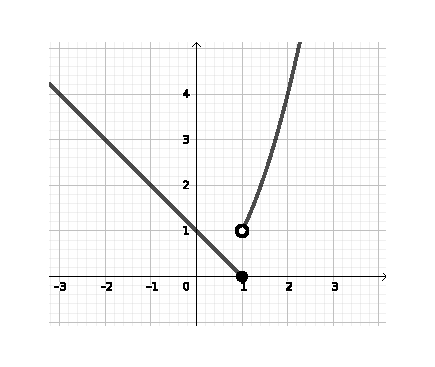
\includegraphics[width=0.95\columnwidth]{T1-2}
  \end{center}
  \end{multicols}
  \item Rewrite $f(x) = \abs{x^2-x-2}$ as a piecewise function (without the absolute value).
  
  \bigskip
  
  With $g(x)=x^2-x-2$, we note that 
  \[
  f(x) =\begin{cases} g(x), & \text{ if } g(x)\geq 0\\ -g(x), & \text{ if } g(x)<0\end{cases}
  \]
  We have $x^2-x-2=(x+1)(x-2)\geq 0$ when either $x\leq -1$ (both factors are negative) or $x\geq 2$ (both factors are positive), and $x^2-x-2<0$ when $-1<x<2$ (when $x+1>0$ but $x-2<0$). Thus,
  \[
  f(x) = \begin{cases}x^2-x-2, & \text{ if } x\leq -1\\
  -x^2+x+2, & \text{ if } -1<x<2\\x^2-x-2, &\text{ if } x\geq 2\end{cases}
  \]
  
  \end{enumerate}


  
\end{document}